\documentclass[notes]{subfiles}

\begin{document}
	\chapter{Applications of Differentiation}
	\addcontentsline{toc}{section}{3.1 - Maximum \& Minimum Values}
	\setcounter{section}{1}
	\fancyhead[RO,LE]{\bfseries \large\nameref{cs31}} 
	\fancyhead[LO,RE]{\bfseries \currentname}
	\fancyfoot[C]{{}}
	\fancyfoot[RO,LE]{\large \thepage}	%Footer on Right \thepage is pagenumber
	\fancyfoot[LO,RE]{\large Chapter 3.1}
	
\section*{Maximum \& Minimum Values}\label{cs31}
	\subsection*{Before Class}
	\addcontentsline{toc}{subsection}{Before Class}
	\subsubsection*{Definitions}
	\addcontentsline{toc}{subsubsection}{Definitions}
		\begin{defn}[Absolute (Global) Extrema]
			\showto{ins}{
				Let $c$ be a number in the domain $D$ of a function $f$.  Then, $f(c)$ is the \textbf{absolute maximum} value of $f$ on $D$ if \fbox{$f(c)\geq f(x)$ for all $x\in D$}; $f(c)$ is the \textbf{absolute minimum} value of $f$ on $D$ if \fbox{$f(c)\leq f(x)$ for all $x\in D$}.\\ \\
				Absolute maxima and minima are also called \fbox{global} maxima/minima (or extrema).
			}
			\showto{st}{
				Let $c$ be a number in the domain $D$ of a function $f$.  Then, $f(c)$ is the \textbf{absolute maximum}\vspace{15pt} value of $f$ on $D$ if \blank{3.5}; $f(c)$ is the \textbf{absolute}\vspace{15pt} \textbf{minimum} value of $f$ on $D$ if \blank{3.5}.\\ \\
				Absolute maxima and minima are also called \blank{1.5} maxima/minima (or extrema).	
			}
		\end{defn}
		\newpage
		
			\begin{ex}
				Below are two graphs.  Identify their absolute maxima/minima, if any exist.  Justify your responses.
			\end{ex}\\
			\begin{minipage}{3in}
				\begin{tikzpicture}
					\begin{axis}[
						every tick label/.append style={font=\small},
						axis x line = middle,
						axis y line = middle,
			    			every axis y label/.style={at={(ticklabel cs:1.15)}},
			    			%ytick = {-4, -2, -3, -1, 1, 2, 3, 4},
						y label style={at={(axis description cs:.47,1.15)},anchor=north},
			    			ylabel = {$f(x)$},
		    				every axis x label/.style= {at ={(ticklabel cs:1)}},
		    				%xtick = {-4,-3,-2,-1,1,2,3,4},
		    				x label style={at={(axis description cs:1.1,.5)},anchor=east},
		    				xlabel = {$x$},
		    				xmin = -2.2, xmax = 2.2
					]
						\addplot[<->,thick, samples = 100, smooth, domain = -2:2] {x^2-2};
					\end{axis}
				\end{tikzpicture}
			\end{minipage}
			\begin{minipage}{3.4in}
				\begin{flushright}
				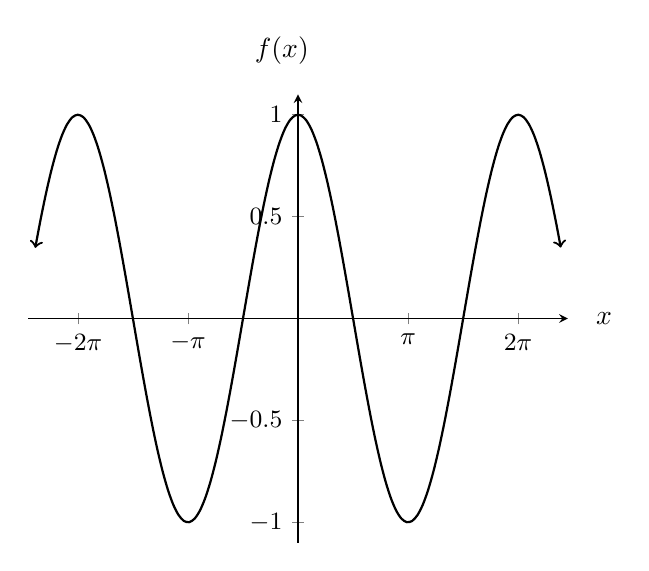
\begin{tikzpicture}
					\begin{axis}[
						every tick label/.append style={font=\small},
						axis x line = middle,
						axis y line = middle,
			    			every axis y label/.style={at={(ticklabel cs:1.15)}},
			    			%ytick = {-4, -2, -3, -1, 1, 2, 3, 4},
						y label style={at={(axis description cs:.47,1.15)},anchor=north},
			    			ylabel = {$f(x)$},
			    			ymin = -1.1, ymax = 1.1,
		    				every axis x label/.style= {at ={(ticklabel cs:1)}},
		    				xtick = {-6.28, -3.14, 0, 3.14, 6.28},
		    				x label style={at={(axis description cs:1.1,.5)},anchor=east},
		    				xticklabels = {$-2\pi$,$-\pi$,0,$\pi$, $2\pi$},
		    				xlabel = {$x$},
		    				xmin = -7.7, xmax = 7.7
					]
						\addplot[<->,thick, samples = 100, smooth, domain = -7.5:7.5] {cos(deg(x))};
					\end{axis}
				\end{tikzpicture}
				\end{flushright}
			\end{minipage}
				
		\begin{defn}[Local Max/Min]
			\showto{ins}{
				The number $f(c)$ is a \textbf{local maximum} value of $f$ if \fbox{$f(c)\geq f(x)$ when $x$ is near $c$}.  $f(c)$ is a \textbf{local minimum} value of $f$ if \fbox{$f(c)\leq f(x)$ when $x$ is near $c$}.
			}
			\showto{st}{
				The number $f(c)$ is a \textbf{local maximum} value of $f$ if \blank{2.5}.  $f(c)$\\ \\ is a \textbf{local minimum} value of $f$ if \blank{3}.\\
			}
		\end{defn}

		\begin{ex}
			Estimate the inputs of any local or absolute extrema.
			\begin{flushleft}
				\begin{tikzpicture}
					\begin{axis}[
						every tick label/.append style={font=\small},
						axis x line = middle,
						axis y line = middle,
			    			every axis y label/.style={at={(ticklabel cs:1.15)}},
			    			%ytick = {-4, -2, -3, -1, 1, 2, 3, 4},
						y label style={at={(axis description cs:.47,1.15)},anchor=north},
			    			ylabel = {$f(x)$},
		    				every axis x label/.style= {at ={(ticklabel cs:1)}},
		    				%xtick = {-4,-3,-2,-1,1,2,3,4},
		    				x label style={at={(axis description cs:1.1,.1)},anchor=east},
		    				xlabel = {$x$},
		    				xmin = -1.5, xmax = 2
					]
						\addplot[<->,thick, samples = 100, smooth, domain = -1.4:1.9] {6*x^4-6*x^3-5*x^2+5*x-1};
					\end{axis}
				\end{tikzpicture}
			\end{flushleft}
		\end{ex}
			\vs{1}

			\newpage

		\begin{question}
			Are local extrema automatically absolute extrema?  Are absolute extrema automatically local extrema?
		\end{question}
			\vs{1}
			
		\begin{ex}
			Identify any local maxes, local mins, absolute maxes, or absolute mins on the graph below.\\
			\includegraphics[scale = .75]{3.1fig1}
		\end{ex}
			\vs{.25}
			
	\subsubsection*{Important Results}
	\addcontentsline{toc}{subsubsection}{Important Results}
		In order to use maxima/minima, some results will be helpful.
		\begin{thm}[Extreme Value Theorem]
			\showto{ins}{
				If $f$ is continuous on a closed interval $[a,b]$, then $f$ attains an absolute maximum value $f(c)$ and an absolute minimum value $f(d)$ at some numbers $c,d$ in $[a,b]$.
			}
			\showto{st}{
				If $f$ is \blank{1.5} on a closed interval $[a,b]$, then \blank{2.3}\vspace{20pt} \blank{5}.
			}
		\end{thm}
			\newpage
		\begin{question}
			Why does the extreme value theorem fail on an open interval?  
		\end{question}
			\vs{1}

		\begin{thm}[Fermat's Theorem]
			\showto{ins}{
				If $f$ has a local maximum or minimum at $c$, and if $f'(c)$ exists, then $f'(c) = 0$.
			}
			\showto{st}{
				If \blank{6.5}\vspace{10pt} then $f'(c) = 0$.
			}
		\end{thm}
		\begin{question}
			Is it true that if $f'(c) = 0$, then $f$ has a local max or min at $c$?
		\end{question}
			\vs{1}
			\newpage

	\subsubsection*{Pre-Class Activities}
	\addcontentsline{toc}{subsubsection}{Pre-Class Activities}
		\begin{ex}
			Give the coordinates for the absolute and local extrema for the function given below.\\
			\includegraphics[scale = 1.25]{3.1fig2}
		\end{ex}
			\vs{.25}
			
		\begin{ex}
			Sketch the graph of a function that has two local maxima, one local minimum, and no absolute minimum.
		\end{ex}
			\vs{1}
		\begin{ex}
			Can we apply Fermat's Theorem to the function $f(x) = |x|$ on the interval $[-5,5]$?  Why or why not? 
		\end{ex}
			\vs{1}
			
		\begin{ex}
			Can we apply the Extreme Value Theorem to the function $f(x) = |x|$ on the interval $[-5,5]$?  Why or why not?
		\end{ex}
			\vs{1}
			\newpage
	
	\subsection*{In-Class}
	\addcontentsline{toc}{subsection}{In-Class}
	\subsubsection*{Critical Numbers}	
	\addcontentsline{toc}{subsubsection}{Critical Numbers}	
		\begin{defn}[Critical Number/Value/Point]
			\showto{ins}{		
				A \textbf{critical number} of a function $f$ is a number $c$ in the domain of $f$ such that \fbox{either $f'(c) = 0$} \fbox{or $f'(c)$ does not exist}.  A \textbf{critical value} is the \fbox{output at a critical input}, namely $f(c)$.  A \textbf{critical point} is the coordinate pair \fbox{$(c, f(c))$}.
			}
			\showto{st}{
				A \textbf{critical number} of a function $f$ is a number $c$ in the domain of $f$ such that\vspace{20pt} \blank{5}.  A \textbf{critical value} is\vspace{20pt} \blank{4}.  A \textbf{critical point} is the coordinate\\ \vspace{5pt} pair  \blank{2}.
			}
		\end{defn}
		\begin{ex}
			Find the critical number(s) of $f(x) = x^3 -3x^2 + 1$.
		\end{ex}
			\vs{1}
			
		\begin{ex}
			Find the critical numbers of $f(t) = t^4 + t^3+t^2 + 1$.
		\end{ex}
			\vs{1}
			\newpage
		\begin{ex}
			For some function $f(x)$, its derivative is given by $f'(x) = \dfrac{100(x-2)^2}{5-x^2}$.  How many critical numbers does $f$ have?  What are they?
		\end{ex}	
			\vs{1}
			
		\begin{ex}
			Find the critical numbers of $f(x) = \cos x$.
		\end{ex}
			\vs{1.5}
	\subsubsection*{Finding Absolute Maxima \& Minima}
	\addcontentsline{toc}{subsubsection}{Finding Absolute Maxima \& Minima}
		In order to find \emph{absolute} extrema on closed intervals, we need to find local extrema and compare the values against the endpoints.  So, finding absolute maxima and minima comes down to the following process:
		\showto{ins}{
			\begin{enumerate}
				\item Find the critical numbers of $f$ on a closed interval $[a,b]$.
				\item Compute the output values at each critical number.
				\item Compute the output values at the two endpoints.
				\item Compare the results from \#2 and \#3.  The biggest output is the absolute maximum, and the smallest output is the absolute minimum.
			\end{enumerate}
		}
		\showto{st}{\\
			\begin{enumerate}
			\setlength\itemsep{25pt}
				\item 
				\item
				\item
				\item
			\end{enumerate}
		}
			\vs{.5}
			\newpage
			
		\begin{ex}
			Locate the absolute extrema for $f(x) = x^3 -3x^2+1$ on the interval $\left[\dfrac{1}{2},4\right]$.
		\end{ex}
			\vs{1}
			
		\begin{ex}
			Locate the absolute extrema for $f(x) = \sin x$ on the interval $[-2\pi,2\pi]$.
		\end{ex}
			\vs{1}
			\newpage
			
		\begin{ex}
			Locate the absolute extrema for the function $f(t) = (t^2-4)^3$ on $[-3,3]$.
		\end{ex}
			\vs{1}
			
		\begin{ex}
			Locate the absolute extrema of the function $f(x) = x + \dfrac{1}{x}$ on $[0.2,4]$.
		\end{ex}
			\vs{1}
			\newpage
			
	\subsection*{After Class}
	\addcontentsline{toc}{subsection}{After Class}
		\begin{ex}
			If $f(x) = 3x^4 - 4x^3 - 12x^2 + 1$, find the absolute maximum and absolute minimium on the interval $[-2,3]$.
		\end{ex}
			\vs{1}
		\begin{ex}
			Find the critical numbers of the function $h(p) =\dfrac{p-1}{p^2+4}$
		\end{ex}
			\vs{1}
		\begin{ex}
			If $a,b$ are positive integers, find the maximum value of $f(x) = x^a(1-x)^b$, for $0\leq x\leq 1$.
		\end{ex}
			\vs{1}
			\newpage
					
		\begin{ex}
			Find the absolute maximum and absolute minimum of the function $f(x) = x\sqrt{3-x}$ on $[-6,3]$.
		\end{ex}	
			\vs{1}
			
		\begin{ex}
			Sketch the graph of a function with two local maxima, one local minimum, and no absolute minimum.
		\end{ex}
			\vs{1}
	\clearpage
\end{document}